\section{Tools and Setup}
\label{sec:tools}
Before analyzing the different tools used in this laboratory, we want to discuss the main goal of this project: managing and configuring a system capable of supporting multi-tenancy and multi-team environments, where each team typically deploys a small number of workloads that scale with the complexity of the service. What we aim to observe are the tools that allow us to share a cluster among different users, while still logically isolating each of them, making it appear as though they are the only ones using the Kubernetes cluster. \\
A Kubernetes cluster consists of a control plane and a data plane. The control plane consists of kubernetes software to manage the back end part of the cluster, we will see technology as \hyperref[subsubsec:kubernetes components]{namespaces}, \hyperref[subsec:resource quotas]{ResourceQuotas}, \hyperref[subsec:resource quotas]{LimitRange} and \hyperref[subsec:access control]{Access Control}. Then, we have the data plane which are composed of worker nodes where tenant workloads are executed as pods (more details in \autoref{subsec:kubernetes}).
\subsection{Tools}
For this project we used a set of high level tools, letting us configure and set up all the process needed. Here there is a brief set of components I used:
\begin{itemize}
    \item \hyperref[subsec:kubernetes]{Kubernetes}.
    \item \hyperref[subsec:Docker]{Docker}.
    \item \hyperref[github]{Github}.
    \item \hyperref[subsec:resource quotas]{Resource Quotas}.
    \item \hyperref[subsec:YAML]{YAML documents}.
\end{itemize}
\label{github}All the images used by me to handle and manage this project can be find in GitHub. Here there are all the needed command to install my repository \cite{FrigoMatteo2025Github}:
\begin{lstlisting}
sudo apt update
sudo apt install git

% Check if it's correctly installed:
git --version
% Clone repository:
git clone https://github.com/FrigoMatteo/Resource-Limitation.git
\end{lstlisting}
Next, I have created a Docker repository where you can install the images I used for the different pods. The installation of them isn't necessary for the completation of this laboratory, since you can easily create your owns one, but for the good of knowleadge I am also sharing this. The images are handled by the docker hub, which is a repository where users can store, manage and share containers with other people. My Docker hub images can be pulled with \cite{FrigoMatteo2025DockerHub}:
\begin{lstlisting}[caption={Pull any image from my repository}]
docker pull matteofrigo1618/repository_name:tag_name
\end{lstlisting}
Now we are going to deep dive on the tools necessary for this laboratory.

\subsection{Docker}
\label{subsec:Docker}
Docker \cite{docker2020docker} is a software platform which allows users to easily create lightweight, portable, and self-contained containers. Docker has also a desktop version, which provides a GUI dashboard letting us see and better manage the containers we have access to, as shown in \autoref{fig:docker desktop}. Unfortunately, Docker desktop has limited functionality instead of CLI, but, in many times, it provides an easy and fast way to check up all your containers. 
\subsubsection{Relation docker-minikube}
The purpose of using Docker is to give Minikube an engine where it can start its containers and, consequently, its pods. It may seem tricky, but in practice, Docker hosts a Minikube container, which then creates and manages other containers through its internal Docker engine. This doesn’t stop here: since we are talking about containers, we can use the images we create or pull from Docker Hub to run inside the Minikube container, which will handle them. \\
Docker images are read-only templates that contain the instructions needed to create a container. They are essentially snapshots of the libraries and dependencies used inside a Docker container, so you will have the same containers I used inside Minikube.
\subsubsection{Docker setup}
Here we provide the procedure to setup Docker. Here you can find original guideline to install it: https://docs.docker.com/engine/install/. 
\begin{figure}[h!]
    \centering
    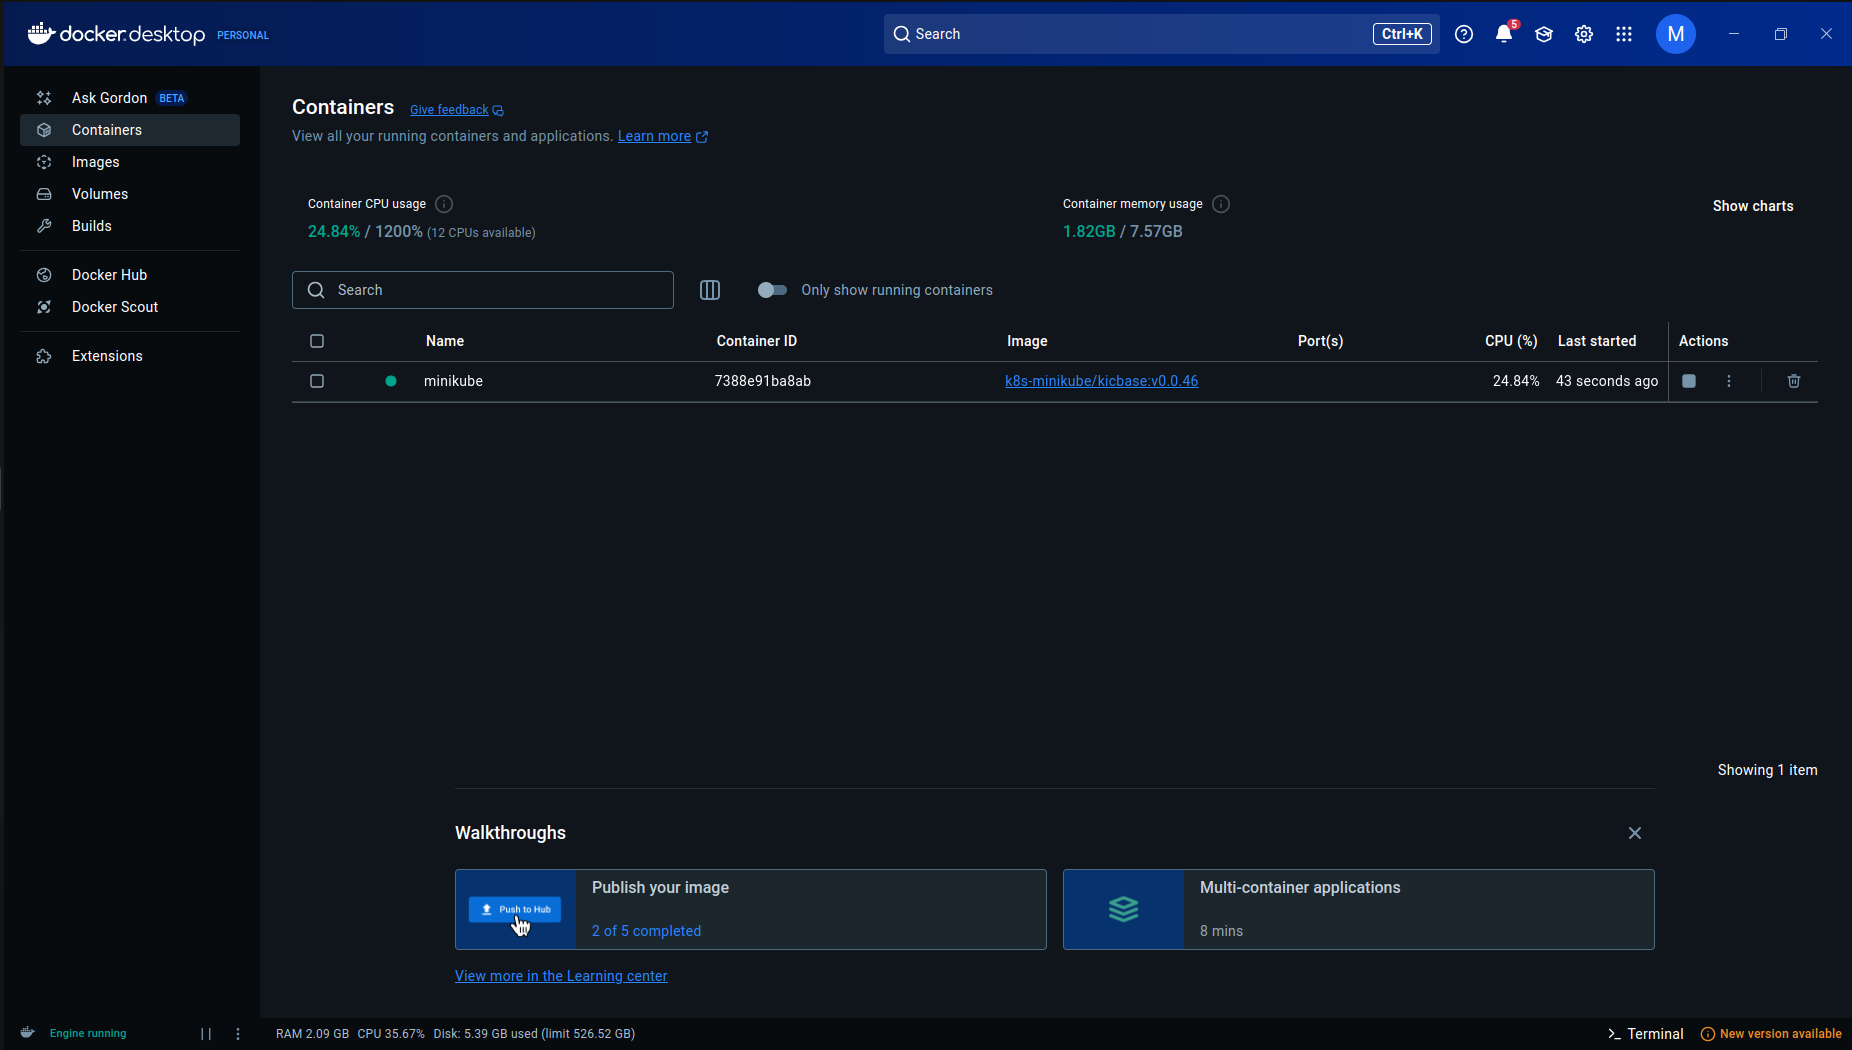
\includegraphics[width=0.7\textwidth]{images/docker_dashboard.png}
    \caption{Docker Desktop Dashboard}
    \label{fig:docker desktop}
\end{figure} \\

\subsection{YAML documents}
\label{subsec:YAML}
We use this kind of documents to describe and define a particular state we want to set in kubernetes. We will use these mechanisms to define resources for the kubernetes deployments, ResourceQuotas and others inside our cluster.

\begin{lstlisting}[language=yaml, caption={Example deployment of four pods, one container each}, label={lst:yaml_default}]
apiVersion: apps/v1         # API version used by kubernetes
kind: Deployment            # Kind of Resource we are creating
metadata:
  name: vite-deployment     # Used to identify the deployment inside the cluster
  labels:
    app: vite
spec:
  replicas: 4               # Number of pods to generate
  selector:
    matchLabels:            # Used to seelct the pods with specific label
      app: vite
  template:
    metadata:
      labels:
        app: vite           # This label must correspond with the one of "selector"
    spec:
      containers:
      - name: vite # Container name
        # Image to use for the container (taken from Dockerhub)
        image: matteofrigo1618/vite_application:v1.0 
        ports: 
          # Each container will have <ip_container>:3000 for cluster's internal communication
        - containerPort: 3000
        resources:
          requests:
            # 250m => 250 millicpu
            cpu: "250m" # request 0.25 core
            memory: "128Mi" # request 128MB of memory
          limits:
            cpu: "500m" # maximum CPU it can take: 0.5 core
            memory: "256Mi" # maximum memory it can take: 256MB
\end{lstlisting}
To apply or delete yaml documents inside the kubernetes cluster, we use the following command:
\begin{lstlisting}[caption={Add or remove YAML document}]
% Apply
kubectl apply -f <file>.yaml
% Delete
kubectl delete -f <file>.yaml
\end{lstlisting}

\subsection{Kubernetes}
\label{subsec:kubernetes}
Here we define Kubernetes \cite{kubernetes2019kubernetes}, which is an open-source container orchestration tool. It helps us orchestrate hundreds of containerized applications in different environments, including both physical and cloud machines. This is a very useful tool, since we don't want to manage all the containers ourselves — they can be complex, time-consuming, and prone to human error during configuration. Kubernetes helps us avoid such problems by handling the containers automatically.
Working with Kubernetes provides the following advantages:
\begin{itemize}
    \item Availability.Applications experience no downtime. Kubernetes supports blue-green deployments.
    \item Scalability. It can easily scale up the number of containers based on user requests, and conversely, scale down when demand is low.
    \item Disaster recovery. Kubernetes includes mechanisms to handle failures by restoring containers to their last known state, or automatically deploying new ones if necessary.
\end{itemize}

\subsubsection{Kubernetes components}
\label{subsubsec:kubernetes components}
Here we introduce the components of Kubernetes. First, we define the cluster, which is made up of multiple nodes, each of which represents a single compute host (virtual or physical machine). Then, we have two types of nodes:

\begin{itemize}
    \item The master node, which serves as the control plane. It manages the other nodes in the cluster. When we use kubectl to communicate with the cluster, we send requests to the master node, which then calls the specific node and operation.
    \item The worker nodes, which are used to deploy, run, and manage containerized applications.
\end{itemize}
As we will see in \autoref{subsec:minikube}, Minikube manages nodes in a different way.
Next, we define the most important components we will use and interact with during this laboratory:

\begin{itemize}
    \item Kubernetes Deployment – These objects are defined by YAML files that declare the desired state we want our application to follow. See an example in \autoref{lst:yaml_default}.
    \item Container – The application that contains our code and runs inside a pod.
    \item Pod – The basic execution unit of a Kubernetes application, which may consist of one or multiple containers.
    \item Namespace – A way to logically group resources (pods, services, etc.) inside a cluster. For example, we can define a namespace for the front-end application, with specific limits and rules, different from those for the back-end application. In addition, many Kubernetes security policies are scoped to namespaces, making them fundamental to services.
    \item kubectl – This is used by developers to communicate directly with the master node to access or send information about the cluster.
    \item Kubelet – Each worker node includes this component, which communicates with the kube-apiserver on the control plane of the master node and receives commands from it.
\end{itemize}

\subsubsection{Minikube}
\label{subsec:minikube}
Minikube is mainly used for testing application in a local machine. I used this component for the sake of the project and the available resources. In fact, minikube is basically a local machine version of kubernetes. In fact, with minikube we can launch a cluster in a single node machine, by having the master and multiple worker node all together, something that it's not possible with the normal kubernetes.
\\[0.5em]
\noindent\textbf{Minikube setup:} 
\vspace{0.2em} \\
Here I consider the installation of minikube for an Ubuntu operating system. In case of errors of fails I suggest you to follow the minikube guideline at https://minikube.sigs.k8s.io/docs/start/. We install the latest minikube stable release on x86-64 Linux.
\begin{lstlisting}
curl -LO https://github.com/kubernetes/minikube/releases/latest/download/minikube-linux-amd64
sudo install minikube-linux-amd64 /usr/local/bin/minikube && rm minikube-linux-amd64
\end{lstlisting}
After doing so, we can use the command to start the minikube cluster:
\begin{lstlisting}[caption={Start minikube command line}]
% We want to specify to use Docker as container engine
minikube start --driver docker
\end{lstlisting}
What you should see it's a screen like in \autoref{fig:minikube start}. It will take some times, since it needs to pull Minikube from the repository, but the next time you will open it, it will be faster.
\begin{figure}[h!]
    \centering
    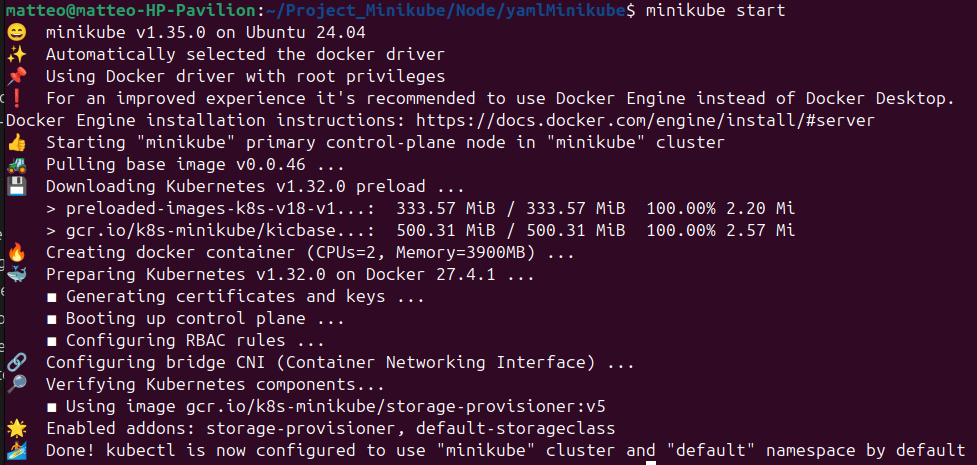
\includegraphics[width=0.65\textwidth]{images/minikube_start.png}
    \caption{Minikube start procedure}
    \label{fig:minikube start}
\end{figure} \\
Now to check if everything is okay, you should be able to send the next line and see the result of the status of minikube:
\begin{lstlisting}
$ minikube status
minikube
type: Control Plane
host: Running
kubelet: Running
apiserver: Running
kubeconfig: Configured
\end{lstlisting}
Make sure everything is running and configured, since these, as previously said, are important component necessary for our system. For more details about the commands and related information about Minikube, I redirect you to the official website: https://minikube.sigs.k8s.io/docs/handbook/.

\subsection{ResourceQuota and LimitRange}
\label{subsec:resource quotas}
Now, we are going to explain why ResourceQuota \cite{kubernetes2025resourcequotas} and LimitRange are fundamental in a project involving Kubernetes.
In the current configuration, any node or pod can use as many resources as it wants. This might be acceptable if we have an abundance of resources, but it becomes problematic in real systems with many pods and containers running simultaneously. This can lead to what is called the "noisy neighbor" problem, where containers compete for and steal resources from each other. A possible solution is to use resource requests and limits for specific containers. An example can be seen in \autoref{lst:yaml_default}, where we define the code to set resource limits for individual containers (not pods). We define:
\begin{itemize}
    \item Request – This is the minimum amount of resources a container is guaranteed. Even if the container doesn't use all those resources, they are reserved and always available.
    \item Limit – This is the maximum amount of resources a container is allowed to use.
\end{itemize}
However, this mechanism alone is not enough. If a container or pod is left unregulated, one pod might consume all the available resources, depriving others that also need them. In this case, we are limiting the resources per container, but not globally per pod. If a team forgets to configure these limits, it can lead to chaos within the cluster.
To ensure a stable and well-managed environment, we use LimitRange and ResourceQuota. These tools are particularly useful in environments where teams may forget to define resource limitations for their applications. That’s why we introduce:
\begin{itemize}
    \item ResourceQuota – This allows us to set resource usage limits per namespace, preventing any single namespace from consuming all the available resources. When distributing resources among teams, the system works on a first-come, first-served basis. See the setup in \autoref{subsec:resourceQuotas}.
    \item LimitRange – Unlike ResourceQuota, which sets quotas at the namespace level, LimitRange defines default resource limits for individual containers within a namespace. See its setup in \autoref{subsec:limitRange}.
\end{itemize}
The cooperation between these two mechanisms provides control and isolation in environments with multiple teams or tenants, especially in shared or cloud-based infrastructures serving multiple customers. In addition, they help developers avoid errors, such as forgetting to set resource limits, which could cause future problems in the cluster.

\subsubsection{ResourceQuotas setup}
\label{subsec:resourceQuotas}
If we work with ResourceQuotas for CPU and memory resources, we enforce that every pod in that namespace sets limits for those resources.
If a resource quota is enforced in a namespace for either CPU or memory, you, and any other clients, must specify either requests or limits for that resource for every new pod you submit, as specified in \autoref{lst:yaml_default}. If you don’t, the control plane may reject the admission of that pod.
One way to enforce this \textbf{automatically and globally}, without relying solely on users to configure it manually, is by using \hyperref[subsec:limitRange]{LimitRange}, which defines default requests and limits for each pod. \\
For example, in a cluster with a capacity of 16 GiB of RAM and 12 cores, if we need to distribute computational resources among different teams, we can describe this configuration using a YAML document, as shown in \autoref{lst:yaml_resourceQuotas_setup}.
First, we need to create the namespace where our ResourceQuota rules will be applied:
\begin{lstlisting}
$ kubectl create namespace <name>
namespace/<name> created
\end{lstlisting}
Then, after succeding in creating the namespaces, we can create the YAML document to launch and apply the ResourceQuotas to the two namespaces:
\begin{lstlisting}[language=yaml, caption={Deployment namespace ResourceQuotas}, label={lst:yaml_resourceQuotas_setup}]
apiVersion: v1
kind: ResourceQuota
metadata:
  name: quota-team
  namespace: <namespace name>
spec:
  hard: # Minimum amount of resources they will have
    pods: "<max pods number>"              # [0, 1, 2, 3..]
    requests.cpu: "<cores number>"         # [0, 1, 2, 3..] = [1000m, 2000m, ...]
    requests.memory: <memory number>       # [100Mi, 200Mi,.., 1Gi, 2Gi..]
    # Maximum amount of resources they can take
    limits.cpu: "<core number>"
    limits.memory: <memory number> 
\end{lstlisting}
Now, if we try to launch an example of deployment inside the namespace, we should see the applied ResourceQuota to the specific environment as shown in \autoref{fig:describe Resource Quotas}.
\begin{figure}[h!]
    \centering
    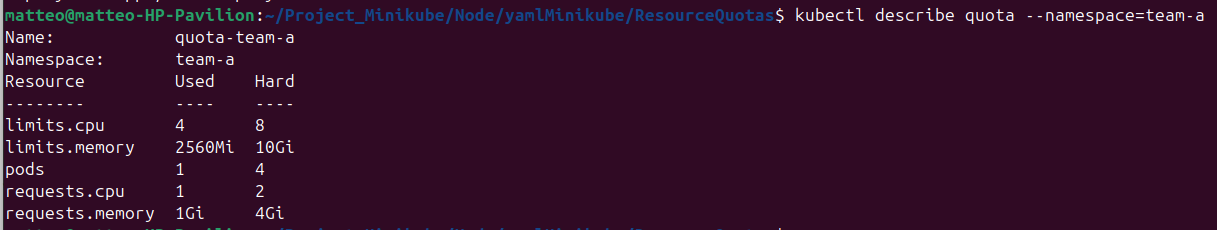
\includegraphics[width=0.7\textwidth]{images/describe_resource_quota.png}
    \caption{Describe Resource Quotas}
    \label{fig:describe Resource Quotas}
\end{figure}

\subsubsection{LimitRange setup}
\label{subsec:limitRange}
By default, containers run with unbounded compute resources in a Kubernetes cluster.
We have seen that by using Kubernetes \hyperref[subsec:resourceQuotas]{ResourceQuotas}, we can restrict the consumption and creation of cluster resources within a specified namespace.
However, within a namespace, a pod can still consume as much CPU and memory as allowed by the ResourceQuotas. So, what we want to add to the cluster is the ability to prevent a single object from monopolizing all available resources within a namespace.\\
This mechanism is the same as the one explained for setting limits and requests on individual pods, such as in \autoref{lst:yaml_default}, but in this case, it will be applied globally to every pod or container within the namespace. The LimitRange object can enforce constraints related to maximum and minimum resource usage, and can also set default requests and limits for compute resources within a namespace for every container or pod.
\begin{lstlisting}[language=yaml, caption={LimitRange Setup}]
apiVersion: v1
kind: LimitRange
metadata:
  name: limit-range-constraints
  namespace: <namespace name>
spec:
  limits:
    # Default values if the container don't specify the limit and request:
  - default: # Defines default limits
      cpu: "<cores number>"         # [0, 1, 2, 3..] = [1000m, 2000m, ...]
      memory: <memory number>       # [100Mi, 200Mi,.., 1Gi, 2Gi..]
    defaultRequest: # Defines default requests
      cpu: "<cores number>"
    # Maximum and minimum values a container can take when initialized
    max:
      cpu: "<cores number>"
      memory: "<memory Mi>" 
    min:
      cpu: "<cores number>"
      memory: "<memory Mi>" 
    type: <type> # [Container, Pod]
\end{lstlisting}
We can see if it's operative by following the procedure in \autoref{fig:describe LimitRange}:
\begin{figure}[h!]
    \centering
    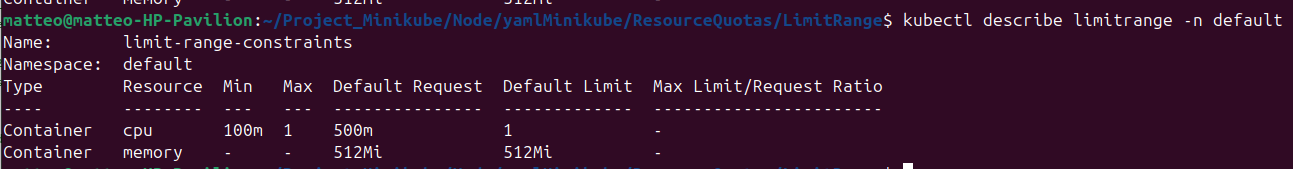
\includegraphics[width=0.8\textwidth]{images/describe_limit_range.png}
    \caption{Describe Resource Quotas}
    \label{fig:describe LimitRange}
\end{figure}

\subsubsection{Possible errors}
\label{subsub:possible errors}
I would pay close attention when creating pods or deployments with ResourceQuota and LimitRange limitations. In fact, when defining the container resources, we must be careful about how much we request. \\
For example, if we consider a setup like \hyperref[lst:yaml_resourceQuotas_setup]{ResourceQuota} with "request.cpu = 2000m", and we define a deployment, such as the one shown in \autoref{example error deployment}, that includes two pods each requesting cpu = 2000m, this will cause issues. The first pod will be created using the requested CPU, but the second one will fail to be created because all available CPU resources (according to the request quota) are already consumed. To allow both pods to be scheduled, we should instead set request.cpu = 1000m, so that both pods can run simultaneously. \\
Remember: we are now setting the minimum amount of resources a pod can use.
Once initialized, both pods can still request additional resources—up to the limit specified in the "limits" section of the YAML document. I would also be careful when defining deployment constraints for all resource parameters.
If you make a mistake, the system may still \textbf{return a success message}, even though the pods or containers were not initialized correctly.
\begin{lstlisting}[language=yaml, caption={Deployment web application with team-a namespace}, label={example error deployment}]
apiVersion: apps/v1
kind: Deployment
**** Deployment configurations ****
spec:
  replicas: 2
    **** Deployment configurations ****
      containers: # ATTENTION IN SETTING CONSTRAINTS
        resources:
          requests:
            cpu: "2000m"
            memory: "1024Mi"
          limits:
            cpu: "4"
            memory: "2560Mi"
\end{lstlisting}
\subsection{Access Control}
\label{subsec:access control}
Access control is one of the most important types of isolation for the control plane part of the kubernetes cluster, since it requires authorization for the operations we perform.
If teams can access or modify each other’s API resources, they can change or disable policies, thereby negating any protection those policies may offer. 
As a result, it is critical to ensure that each tenant has access only to the namespaces they need—and nothing more. This is known as the \textbf{Principle of Least Privilege}. \\
Role-Based Access Control (RBAC) is commonly used to enforce authorization in the Kubernetes control plane. In a multi-team environment, RBAC must be used to restrict tenants’ access to the appropriate namespaces and to ensure that cluster-wide resources can only be accessed or modified by privileged users, such as cluster administrators. \\ 
This policy is mainly used to restrict access to kubernetes API if the tenants ask for specific pods/deployment to the administrator to perform read or write operations to the configurations of the kubernetes cluster. We can divide these components into three categories:
\begin{itemize}
    \item Identity. They can be users, which are externally defined, or Service Accounts, that are entities managed by kubernetes for the pods.
    \item Role. The role defines the group of permission inside a specific namespace. We can also have RoleCluster, which are the set of rules for a cluster or group of namespaces.
    \item Role Binding. We assign a Role or a RoleCluster to one or multiple users/group.
\end{itemize}
\subsubsection{Identities}
We have two categories of identities: users and Service Accounts. A user is an external identity, which is not managed by the Kubernetes cluster, but it is still possible to use it and authenticate via certificates such as X.509. Different users have specific permissions to access or modify the entire cluster through tools like kubectl or the dashboard commands, as we have seen so far, with possible restrictions based on policies. However, for the purpose of multi-tenancy, users do not fit well within the structure. This is better managed by Service Accounts, which can represent either a user (human) or an application, providing an identity for processes running inside a pod. Using Service Accounts, we can monitor, scale up, or modify the resources available within our namespace. Moreover, unlike users, Service Accounts are managed (created, modified, or monitored) by Kubernetes itself, having their own objects that we can reference. We can create a Service Account using the following YAML code:
\begin{lstlisting}[language=yaml, caption={Service Account creation}, label={lst:service_account_creation}]
apiVersion: v1
kind: ServiceAccount
metadata:
  name: <name Service Account>
  namespace: <name Namespace>
\end{lstlisting}
\subsubsection{Role and ClusterRole}
A Role or ClusterRole contains rules that represent a set of permissions. A Role always sets permissions within a particular namespace; when you create a Role, you have to specify the namespace it belongs in. If we want to define a role cluster-wide, we use a ClusterRole. We can create a Role or Cluster role with the following YAML commands:
\begin{lstlisting}[language=yaml, caption={Role or Cluster Role creation}, label={lst:service_account_creation}]
apiVersion: rbac.authorization.k8s.io/v1
kind: <Role> # [Role, ClusterRole]
metadata:
  namespace: <name Namespace>
  name: <Name of the Role>
rules:
- apiGroups: [<Api Group>]
  resources: [<resources>] # [pods, services, nodes, deployments, etc..]
  verbs: [<constraints>] # [get, list, delete, watch, create, update, etc..]
\end{lstlisting}
Inside the YAML document presented, we also define the "apiGroups". These are used by kubernetes to group and organize the resources inside his API REST. We have different mods, the main one is empty quotation, which include the APIs for resources as pods, services configmap and others. So, based on the apiGroup we choose, we will have different resources available.
\subsubsection{Role and Cluster Binding}
A role binding grants the permissions defined in a role to one or more users or Service Account. A RoleBinding grants permissions within a specific namespace whereas a ClusterRoleBinding grants that access cluster-wide. Here there is how we define it:
\begin{lstlisting}[language=yaml, caption={RoleBinding creation}]
apiVersion: rbac.authorization.k8s.io/v1
kind: RoleBinding
metadata:
  name: <name> # Name we want to give to binding
  namespace: <name Namespace>
subjects:
- kind: ServiceAccount # In case you want to bind a user => "User"
  name: <name of Service Account>
  namespace: <name Namespace>
roleRef:
  kind: <type of Role> # [Role, ClusterRole]
  name: <name of the Role>
  apiGroup: rbac.authorization.k8s.io
\end{lstlisting}


\subsection{Network Policies}
\label{subsec:network policies}
Inside a cluster, by default, each pod can talk to any other pod inside it. So a tenant, in this case, could communicate with resources of other tenants. For this reason we want to limit the communication with network rules inside the cluster. For the purpose of our laboratory, we will focus only on the isolation of the namespace, since deeper isolations of specific pods or resources are dependent based on the application we want to create/install inside our namespace. \\
For example, there can be rules where the Front-end pod of a web application can talk only to the back-end pod, not permitting direct communication with a database, but forcing it to communicate with the back-end for specific kind of operations. \\
In addition, this can also protect us against any possible infections of pods inside the kubernetes cluster, without permitting an infected pod to communicate and propagate to other resources of other namespaces. Now, I am going to show you only a namespace isolation between multiple tenants:
\begin{lstlisting}[language=yaml, caption={Network policy setup}]
apiVersion: networking.k8s.io/v1
kind: NetworkPolicy
metadata:
  name: <policy name you want>
  namespace: <name namespace>
spec:
  # podSelector => {} => affect all pods of the namespace
  # If we want to select specific pods => {podName1, podName2..}
  podSelector: {}
  policyTypes:
  - Ingress # Control traffic in ingress
  ingress:
  - from:
    - podSelector: {} # This imply we consent traffic only from our namespace
\end{lstlisting}
As we saw, we only limit traffic going inside our namespace, but the pods inside can still communicate with namespace's resources of the cluster or external cluster. In addition, this policy is applied only for internal cluster communications, so it acceptes any incoming traffic from outside the cluster.